\section{完成情况及性能参数}
\subsection{整体介绍}
基础相机、网络及HDMI显示链路已有历史实板记录。当前两来源模型完成整数参考、RTL、720p视频调度和物理实现检查，于2026年10月21日11:37由TD6.2成功下载PH1P35MDG324主板SRAM。用户随后反馈实拍效果较前版更好，并表示已自行完成Flash烧录；此反馈属于定性实板观察，尚无带标签相机数据的独立定量准确率、当前HDMI验收或断电冷启动记录。

当前主工程位于camera processing unit目录。活动硬件树为\path{hardware/mainboard/}和\path{hardware/hdmi/}。整理前构建使用既有主板工程，构建时.al哈希保存在冻结资产；整理后.al中的文件路径已随目录调整，因此不再把当前工程文件写成“字节不变”。最终候选bit、模型和非路径源码的身份由清单核对；历史构建路径与当前位置通过映射关联。旧bit、源码和模型仍在\path{yolo/wbc_bccd/baseline/}保留。

\Needspace{10\baselineskip}
\subsection{工程成果}
\subsubsection{机械成果}
完成显微镜摄像头支架V10的三维设计，形成显微镜采集与竖直演示两套装配模型，提供六种零件的可编辑模型及STL打印文件。底座、立柱与托座实现开发板承放、排线整理和摄像头定位；遮光后盖采用一体式周圈台阶结构。已完成模型闭合性、几何配合和STL检查，打印后的承载、遮光及合焦效果需结合实物试装确认。\cite{mechanical}

\subsubsection{电路成果}
主板形成 MIPI 接收、RAW10 解包、ISP、PID 曝光控制、全帧RGB160采样、量化联合检测分类、单目标身份与类别确认、框与类型叠加、双口发送和网络命令通路；子板维持协议接收、帧重组、三缓冲显存、DQS 读回与 HDMI 通路。本轮资源与时序统计包含整个主板，不是独立 CNN 核的综合估计。

\begin{table}[htbp]\centering\small
\caption{当前两来源模型位流的完整布线资源与时序}
\begin{tabularx}{\linewidth}{|L{3.2cm}|Y|}
\hline\tablehead 指标 & 当前实现结果\\\hline
Slice & 19016/21216，89.63\%\\\hline
ERAM20K & 94/108，87.04\%\\\hline
DSP & 35/40，87.50\%\\\hline
setup WNS & +0.102 ns\\\hline
hold WNS & +0.020 ns\\\hline
时序结论范围 & 既有约束下的最终物理实现摘要\\\hline
\end{tabularx}\label{tab:resource}
\end{table}

主板采用PH1P35MDG324，工具为TD 6.2.168116；像素处理与推理为100 MHz，GMII发送为125 MHz。表\ref{tab:resource}依据当前保留的\code{build_result.json}与发布摘要，Slice剩2200个，ERAM剩14块，DSP剩5个。原始\code{route.area}、\code{route.timing}及部分运行日志已在目录整理时清理，本文不将其列为现存可复查文件。摘要中的正裕量表示既有约束下的静态时序通过，新增网络或修改路径仍需重新实现。\cite{resource,timing}

子板沿用已有显示工程，RGMII采样、DDR控制、显示像素时钟与串化时钟在约束中显式组织，异步传递由同步器或FIFO完成。本次作品报告更新未重新构建或下载子板；其验证结果按历史资料解释。\cite{hdmicolor}

\subsubsection{软件成果}
PC GUI 支持原样收图、完整 RGB 帧保存、七模式切换、轮廓参数与白平衡控制。实时细胞检测、取图、分类和文字不在 PC 运行，视频内的框和类型来自主板 RGB；通信统计位于图像外。控制参数以请求、应答、提交和查询组成事务，界面显示确认值；接收线程与状态线程独立运行，避免控件操作阻塞收图。

离线工具完成掩膜转整细胞框、去重与负样本生成、模型训练、量化感知训练、ROM 导出、整数参考推理、网络向量生成及 RTL 记分板检查。训练与评估在开发电脑执行，不参与相机实时推理链路。构建与下载记录核验源码、模型和bit哈希，已核实的成功记录为PH1P35主板SRAM下载。后续本机自动Flash操作校验失败，用户自行烧录成功的反馈另行记录；本轮未重新下载HDMI子板。\cite{gui,interface,training}

\Needspace{9\baselineskip}
\subsection{特性成果}
\lead{图像与自动调节功能}
上板系统提供 720p30 图像输出，七种模式可运行时切换；白平衡支持预设、色温、手动和自动模式；AE 使用曝光优先的 PID 和全局数字增益。图像模式、白平衡与数字增益在帧边界提交，曝光设置通过传感器事务执行。上位机显示实际目标、设置确认和链路健康，便于区分用户设置、已提交状态及图像反馈。

控制模型对明暗场、数字增益分配、高反差、交替亮度和确认延迟进行检查。两帧与四帧窗口切换受误差阈值控制；达到死区后停止调节，失败事务后重新收集统计。已有完整视频 RTL 用例覆盖 460 帧，核对帧身份、长度、非黑输出与流健康；这些属于模型和仿真检查，不能代替本轮新权重位流的相机实拍结论。\cite{pid}

\lead{网络与显存一致性}
既有发布摘要记录主板42项RTL、两组完整网络包校验和38项Python测试通过。本次仅更新报告，未重跑这些硬件回归。网络包由独立 CRC/IP/UDP 校验器解析，避免发送端与检查端共用同一错误计算过程。历史子板验证从GMII/RGMII输入到重组、DMA、DDR引脚和HDMI编码器前RGB分层核对，验证范围延伸到实际数据显示的位置。

\begin{table}[htbp]\centering\small
\caption{子板显示链路的历史量化验证（本次未重跑）}
\begin{tabularx}{\linewidth}{|L{3.1cm}|Y|}
\hline\tablehead 检查对象 & 结果及条件\\\hline
协议与重组 & 历史8场景回归通过，覆盖完整帧、丢包、重复、乱序和坏FCS等\\\hline
全分辨率工况 & 历史1920包/帧、11帧向量逐字节核对\\\hline
仲裁与刷新压力 & 历史压力扫描包含2 ms总线黑窗注入\\\hline
OSD落点 & 历史账本逐像素diff=0，图案与logo区域分别核对\\\hline
本次范围 & 核对现存文档与源码；未重跑子板仿真或重新上板\\\hline
\end{tabularx}
\end{table}

表中结果来自保留的子板专题文档，反映当时的回归记录。协议和像素仿真不覆盖板上全部电气采样裕量，实际工作还依赖RGMII采样相位、DDR引脚约束、布线和供电条件。\cite{hdmicolor}


\lead{联合检测分类的整数与视频验证}
本轮两来源模型接入的14张自然图及派生负图覆盖全部五类输出。每张逐项核对十层整数输出、6400个首层特征字、3000个logit和最终框、类型、分数，与独立整数参考完全一致。五项组件测试覆盖全帧采样与抽帧、top20与NMS、身份与类别确认、单目标选择及英文全称；三项既有跟踪回归包括90帧五目标参考策略。英文全称边缘位置和17941个文字像素有单独核对。

两种完整720p30时序各输入六帧，分别使用突发输入与每像素三拍、每行4444拍的输入节拍，验证15 Hz支路完成三次检测，非推理帧保持结果。第3至6帧有边框，第5至6帧有确认后的类别文字，更新中没有临时清空框。组件另测两次漏检保留、第三次撤框、配置切换、超时及重新出现确认。最慢节拍从采样起点到提交6295080拍，约62.95 ms。仿真证明数值与调度，不等同相机实测15 Hz或实拍零闪烁。42项原视频RTL、两项包完整性及38项Python回归均重新通过。\cite{yoloreport}

\lead{历史方案与当前报告范围}
早期CellNet32与中心窗口分类、单WBCAtt+实验均属于历史方案。单来源模型曾在同源公开TEST获得92.39\%联合macro-F1，但出现实拍空场景误检并被撤回；该结果不能写作当前部署成绩。当前模型是\code{wbc_bccd160_devcam_20261021}，采用两来源训练及新的objectness评分。下文只以当前冻结资产统计数据与模型表现，历史失败用于说明引入真实背景域和开发校准的原因。\cite{repo,twosource}

\lead{两来源数据与质量控制}
WBCAtt+以整细胞掩膜外接框提供五类和定位监督；BCCD仅提供白细胞定位监督，类别保持-1并屏蔽分类损失。原图和派生背景裁图数量分别统计，派生图继承父图划分。解码RGB160跨划分精确重复为零，但没有患者级独立性证明；TEST在前期实验中已查看，本轮只作为已使用测试集回归。\cite{wbcatt,datarepo,training}

\begin{table}[htbp]\centering\small
\caption{当前模型冻结数据划分（原图 / 派生负裁图）}
\begin{tabularx}{\linewidth}{|L{2.2cm}|Y|Y|}
\hline\tablehead 划分 & WBCAtt+ & BCCD\\\hline
TRAIN & 6021 / 6020 & 205 / 270\\\hline
VAL & 1010 / 1010 & 87 / 122\\\hline
已使用TEST & 3017 / 3017 & 72 / 99\\\hline
\end{tabularx}
\end{table}

\begin{center}
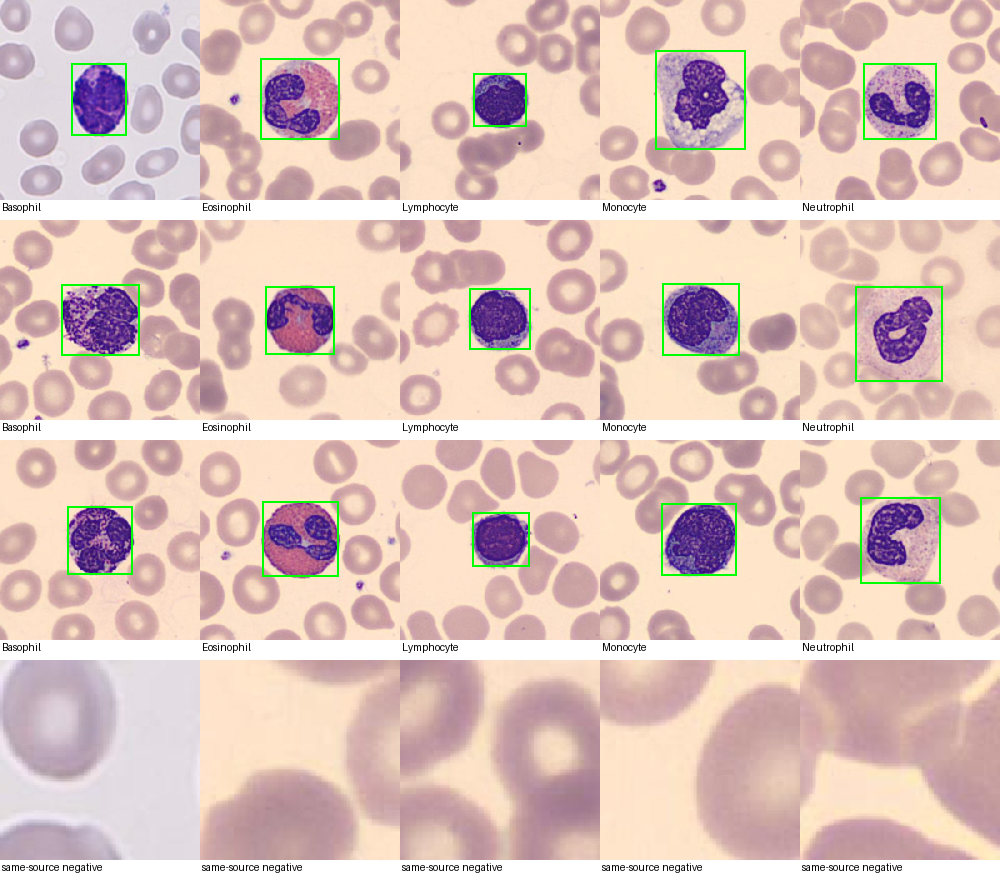
\includegraphics[width=0.82\linewidth]{images/wbcatt_training_preview.png}
\captionof{figure}{仅取TRAIN的五类标注与同源负裁图示例；绿色框来自整细胞掩膜，不是网络预测或主板实拍。}
\end{center}

\lead{WBCAtt+与BCCD两来源重训及当前部署}
本轮仅使用两套采集数据，不加入Raabin图像或Raabin训练权重。初始化来自从随机权重开始的WBCAtt-only FP32 checkpoint。WBCAtt+的TRAIN/VAL/TEST原图为6021/1010/3017，派生背景裁图为6020/1010/3017；BCCD原图为205/87/72，负裁图为270/122/99。BCCD只使用WBC框，五类标签保持-1并屏蔽分类损失；没有给其制造五类伪标。派生样本随原图划分，实际RGB160跨划分精确重复为零，不证明患者独立性。

完成120轮FP32与80轮QAT、60轮低照正样本QAT，最后40轮只训练objectness输出；按五类、BCCD及负样本分层采样。mosaic只作用于有五类标签的正图槽，避免减少空图比例。程序化纯色、暗场、矩形、渐变和噪声作为增强。首轮两来源模型空场景已无框，但旧细胞拍屏图仍漏检，提亮诊断说明存在曝光差异；追加低照正图与拍屏比例，并重放原始明亮细胞真值。固定相机增强VAL来自VAL父图，不是独立相机测试。checkpoint由VAL选择，权重冻结后原仅VAL阈值0.95仍漏旧图；部署改用公开/固定增强VAL及用户给过的有、无细胞截图，在0.40至0.95、步长0.025网格进行开发校准，选定52020/65025。截图像素和未知类型没有用于训练，但截图用于阈值选择，不能再称仅VAL校准或独立相机验收。TEST未参与选择；它在前次实验已被查看，本次只称已使用测试集回归。

\begin{table}[htbp]\centering\small
\caption{当前两来源整数模型结果（\%，框IoU$\geq$0.5）}
\begin{tabularx}{\linewidth}{|Y|r|r|}
\hline\tablehead 指标 & VAL & 已使用TEST回归\\\hline
WBCAtt+联合macro-F1 & 89.81 & 91.40\\\hline
WBCAtt+框与类型正确召回 & 95.45 & 96.75\\\hline
BCCD定位召回 & 100.00 & 98.59\\\hline
BCCD定位精确率 & 93.55 & 88.61\\\hline
WBCAtt+负图有框比例 & 3.47 & 2.78\\\hline
BCCD空图有框比例 & 4.07 & 6.80\\\hline
Basophil & 90.00 & 94.57\\\hline
Eosinophil & 94.12 & 95.00\\\hline
Lymphocyte & 81.99 & 82.99\\\hline
Monocyte & 89.26 & 90.60\\\hline
Neutrophil & 93.69 & 93.84\\\hline
\end{tabularx}
\end{table}

表中五个英文类别行是各类联合F1，不是只分类准确率；联合正确还要求定位IoU达标。两组1024张程序空场景分别误检18张（1.76\%）及8张（0.78\%）。第一组未达到原1\%目标，原失败记录保留；两组均低于2\%工程试验界限。2\%是看到结果后的工程上板选择，不是事先定义的精度目标。人工压力图不能代表真实相机分布，原图派生负样本仍有误检；本轮按工程试验范围解释，后续用户自行烧录Flash也不改变统计验收范围。12张纯色与给过的室内图无框，旧细胞图能定位但类型真值未知，且截图已用于开发校准。最终对每张空图最强锚框施加背景损失，仅调整三路objectness滤波器，前九层及框/类型参数逐项保持；检测与五类argmax解耦。RTL执行新评分，未新增分类器或上位机算法。

14张自然与派生图完成十层整数对拍；另对黑、灰、白、用户室内图和历史细胞图完成五次整网RTL回放，最终框、类别、分数及逐层结果均与参考一致。五项组件、三项原跟踪、两种720p30完整视频仿真，以及42项既有RTL、两项包完整性、38项Python重新通过。新bit最终时序通过，并核验TD6.2识别PH1P35MDG324、芯片校验成功、Tcl catch=0及download同步结束。本机核实的成功下载为主板SRAM；用户随后报告实拍改善及自行完成Flash烧录，定量实拍精度与HDMI效果尚无独立验收。\cite{twosource}

\begin{center}
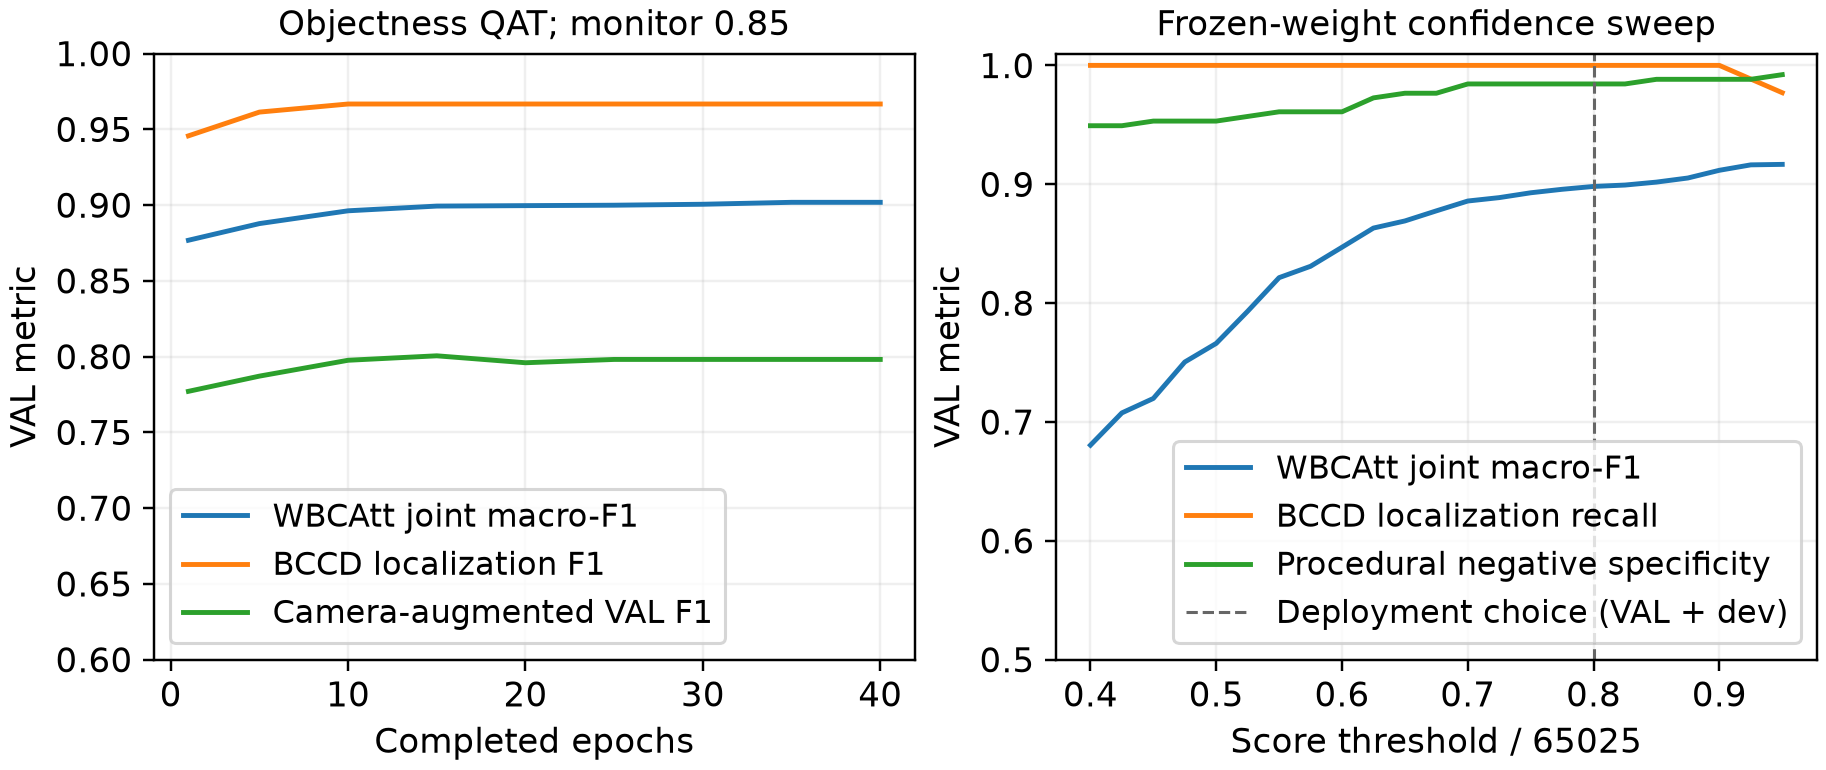
\includegraphics[width=0.98\linewidth]{images/two_source_training.png}
\captionof{figure}{仅objectness追加训练与开发阈值校准。左图固定0.85阈值监测，右图在冻结权重后扫描，虚线为结合公开验证及用户开发截图选定的部署阈值。程序空图特异性不是相机域性能。}
\end{center}



\begin{center}\small
\captionof{table}{截至2026年10月21日的验证与部署证据范围}
\begin{tabularx}{\linewidth}{|L{3.0cm}|Y|}
\hline\tablehead 类别 & 当前记录及适用范围\\\hline
模型与RTL & 冻结评估、向量和组件摘要通过；说明整数计算与调度一致\\\hline
资源与时序 & 最终候选完整主板物理摘要通过；本次未重新布局布线\\\hline
SRAM下载 & TD6.2成功摘要，候选bit哈希已核对\\\hline
Flash部署 & 本机自动操作失败；用户反馈手动完成，烧录文件身份未独立核验\\\hline
实拍与HDMI & 用户定性反馈实拍改善；定量精度、当前HDMI与冷启动待独立核验\\\hline
本次文档检查 & 核对活动RTL、模型/bit哈希与现存摘要；双遍编译并逐页检查PDF\\\hline
\end{tabularx}
\end{center}

\lead{运行状态与测量口径}
图像完整率表示一个视频帧所需的包是否全部收到，需结合 RAW 组数、输出像素数和累计流错误共同判断。FPGA 计时基准为 100 MHz，采集时间起点为帧首事件，不能直接等同于未知的光学曝光起点；PC 的拼帧时间使用单调时钟，上位机提交图像也不等同于显示面板发光时刻。

网络线速、DDR 带宽、CNN 周期和静态时序分别描述传输预算、存储访问、计算耗时和受约束路径裕量，不能直接相加替代从曝光到显示发光的实测延迟。本轮两来源模型已于2026年10月21日11:37通过TD6.2下载主板SRAM；随后收到用户实拍改善及手动Flash烧录完成的反馈。候选bit已核对SHA-256，但用户手动写入的Flash文件身份与断电冷启动未独立核验。本轮新位流SHA256为
\begin{center}\footnotesize
\texttt{5bc2dfee5ef0980b69b3749871bcd768298c5b37af3dcdb67af45930c8ceff58}
\end{center}
旧已验证bit和模型保持归档。本机自动Flash尝试在逐页编程/校验阶段后报\code{PRG-8000: get tdo buffer failed}，Tcl catch=1；该操作不记作成功。用户手动烧录反馈单独保留。后续需在带真值的相机场景记录误检、漏检、类别跳变、WAIT及响应时间；程序下载与用户定性反馈不能替代定量验收。\cite{twosource,programming}
